\documentclass[12pt, letterpaper]{report}
\usepackage{graphicx}
\usepackage{hyperref}
\usepackage{amssymb}
\usepackage{amsmath}
\usepackage{float}
\usepackage{mathtools}
\usepackage{enumitem}
\usepackage[margin=1in]{geometry}
\usepackage[figurename=Figura]{caption}
\title{Actividad: Argumentación detallada sobre el Uso de la Ley de Gauss en Coordenadas Esféricas}
\author{Juan Pablo Guerrero Escudero A01706810}
\date{15 abril, 2024}
\begin{document}
\maketitle
\subsection*{Introducción}
Al analizar situaciones electrostáticas, un componente importante es el campo eléctrico generado por una carga puntual, ya que 
gracias a él podemos observar los efectos en el espacio por medio de la fuerza eléctrica que sienten las cargas de prueba en sus alrededores. Para ésto, es muy común 
utilizar la Ley de Gauss, ya que gracias a ella podemos, por medio de la simetría de un sistema electrico, simplificar 
para hacer los cálculos más fáciles. Como funciona es que, dada una distribución de carga, la encerramos con una superficie 
Gaussiana, la cuál nos permite observar la relación entre el campo eléctrico en todos los puntos de la superficie, y la carga total encerrada por ella. \\
En otras palabras, la Ley de Gauss nos dice que el flujo total eléctico que pasa por cualquier superficie cerrada es proporcional a la carga total neta adentro de 
ésta. Por lo tanto, en éste reporte se analizarán a detalle dos situaciones: Cuando la superficie gaussiana es menor en radio a la distribución de la carga, y cuando la 
superficie gaussiana es mayor en radio a la distribución de la carga. 
\subsection*{Desarrollo}
En primer lugar, con la Ley de Gauss podemos determinar el campo eléctrico cuando la superficie Gaussiana encierra una parcialidad de la carga. 
\begin{figure}[H]
    \centering
    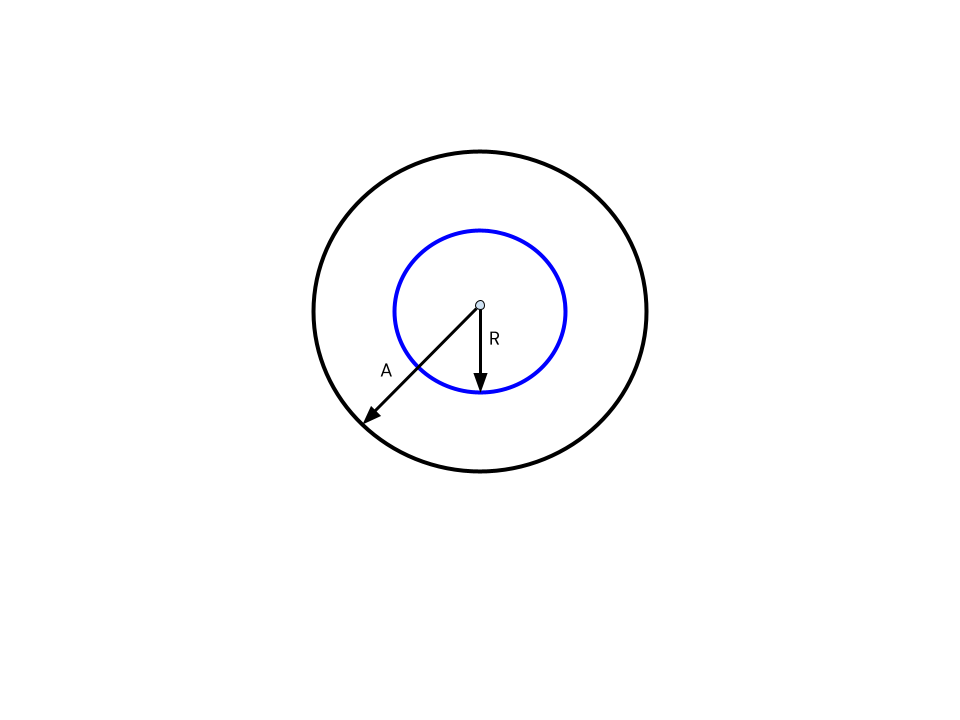
\includegraphics[height = 8cm]{2024-04-18_Diagrama1_ActividadCargas.png}
    \caption{Diagrama de situación donde $R\leq A$. }
    \label{fig:fig1}
\end{figure}
En el diagrama \ref{fig:fig1} se observa la situación en donde la superficie gaussiana, que en éste caso es una esfera, tiene radio $R$, mientras que el radio de la carga 
analizada es $A$, y se cumple que $R \leq A$, es decir, la superficie gaussiana se encuentra dentro de la esfera de la carga. Además, durante todo el proceso se usa el sistema de 
coordenadas esféricas $(\hat{a}_r, \hat{a}_\theta, \hat{a}\phi)$. Ésto debido a que, para que se pueda utilizar Ley de Gauss, se tienen que cumplir 3 condiciones: 
\begin{enumerate}
\item Tiene que haber simetría en la distribución de la carga. 
\item Se tiene que crear una superficie imaginaria que encierre la carga o una parcialidad, la cuál se llama "Superficie Gaussiana". 
\item El campo eléctrico debe ser perpendicular o tangencial a la superficie gaussiana. 
\end{enumerate}
Si se posiciona la carga en el centro de la esfera (superficie Gaussiana), el campo eléctrico se produce de manera radial, por lo que para que siempre sea perpendicular 
a la superficie Gaussiana, se usa una esfera, y por lo tanto las coordenadas esféricas ya que facilitan los cálculos. En las coordenadas esféricas, $\hat{a}_r$ representa el radio de la 
superficie Gaussiana, que va desde $0$ a $r$, $\hat{a}_\theta$ va desde $0$ a $\pi$, y $\hat{a}_\phi$ va desde $0$ a $2\pi$. \\ 

Ahora, la ley de Gauss dice lo siguiente: 
\begin{align}
Q_{enc} &= \oint_S \epsilon_0\vec{E}\cdot d\vec{S} \label{eq:eq1}\\
Q_{enc} &= \int_V \rho_v dv\label{eq:eq2}
\end{align}
Básicamente, nos dice que, de acuerdo a la ecuación \ref{eq:eq1}, la carga encerrada $Q_{enc}$ es igual a la integral de superficie 
cerrada de la constante $E_0$ multiplicada por el campo eléctrico $\vec{E}$, multiplicado por el diferencial de superficie, que es 
$d\vec{s} = (r^2\sin \theta d \theta d \phi \hat{a}_r)(r\sin \theta dr d\phi \hat{a}_\theta)(rdrd\phi \hat{a}_\phi)$. Básicamente, el diferencial 
de superficie $d\vec{s}$ representa el diferencial del área de superficie, que describe un área infinitesimalmente pequeña de la superficie Gaussiana. 
En éste caso, $d\theta$ representa un cambio infinitesimal en $\theta$, medido en el eje $Z$ positivo. Después, $d\phi$ representa igualmente un 
cambio infinitesimal en el ángulo $\phi$, medido en el eje X positivo. Y por lo tanto, la expresión $d\vec{s}$ descompone el diferencial de superficie en 
sus componentes a lo largo de sus tres direcciones $(r, \theta, \phi)$. \\ 

También, la ecuación \ref{eq:eq2} obtiene directamente el total de la carga encerrada al calcular una integral de volumen de $\rho_v$, o densidad de volumen, 
multiplicado por el diferencial de volumen $dv = r^2\sin \theta dr d\theta d\phi$, el cuál es un valor escalar. que representa el cambio infinitesimal de volumen en el espacio. \\ 

Usando éstas ecuaciones con las restriccones del diagrama \ref{fig:fig1}: 
\begin{align}
Q_{enc} &= \int_V \rho_v dv \\
Q_{enc} &= \rho_v \int dv \\ 
Q_{enc} &= \rho_v \int_{0}^{r}\int_{0}^{\pi}\int_{0}^{2\pi}(r^2\sin(\theta)dr d\theta d\phi) \label{eq:eq3} \\ 
Q_{enc} &= \rho_v\int_{0}^{r}(r^2dr)\int_{0}^{\pi}(\sin(\theta)d\theta) \int_{0}^{2\pi}(d\phi) \label{eq:eq4}
\end{align}
Como la integral de volumen es una integral triple, se puede separar el diferencial de volumen $d_v$ en 3 integrales, una por cada 
componente de éste $(dr, d\theta, d\phi)$ en la forma de la ecuación \ref{eq:eq3}. Cabe destacar que la integral para el radio, va de $0$ a 
$r$, debido a que el radio de la superficie crece hasta llegar al radio de la carga $a$. A continuación se resuelve la integral \ref{eq:eq3}: 
\begin{align}
Q_{enc} &= \rho_v[(\frac{r^3}{3}\Big |_0^r)(-\cos(\theta)\Big |_0^\pi)(\phi \Big|_0^{2\pi})]\\
Q_{enc} &= \rho_v[[\frac{r^3}{3}-0][-(-1-1)][2\pi - 0]] \\ 
Q_{enc} &= \frac{4}{3}\pi r^3 \rho_v \label{eq:eq5}
\end{align}
Por lo tanto, al evaluar la integral triple de acuerdo al Teorema Fundamental del Cálculo, la fórmula para la carga encerrada para todo $r\leq a$ es la ecuación 
\ref{eq:eq5}. Cabe destacar que en la ecuación \ref{eq:eq3}, se realizan tres integrales, y el diferencial de volumen es un escalar. 

Como queremos determinar el campo eléctrico en ésta situación, conviene realizar la integral de superficie cerrada en la ecuación \ref{eq:eq1}, para posteriormente igualar éste resultado con 
la ecuación resultante de la integral de volumen, ecuación \ref{eq:eq5}, y así obtener una fórmula para el campo eléctrico. A continuación se muestra éste proceso:
\begin{align}
Q_{enc} &= \oint _S \epsilon_0 \vec{E} \cdot d \vec{S} \\
Q_{enc} &= \epsilon_0 \int Er^2(sin(\theta)d\theta d\phi) \\ 
Q_{enc} &= \epsilon_0 Er^2 \int_{0}^{\pi} \sin(\theta) d\theta \int_{0}^{2\pi} d\phi \\ 
Q_{enc} &= \epsilon_0 Er^2 [-(-1-1)2\pi]\\
q_{enc} &= 4\pi r^2 \epsilon_0 E \label{eq:eq6}
\end{align} 
En el proceso anterior, se resuelve la integral de superficie, la cuál resulta en la ecuación \ref{eq:eq6}, que nos da 
la carga encerrada en términos del radio de la superficie Gaussiana y la magnitud del campo eléctrico. En primer lugar, es importante notar que 
de realizar el producto punto de $\vec{E} = E\hat{a}_r$ y el diferencial de superficie 
$d\vec{s}$, solo permanece el término en el diferencial $r^2\sin\theta dr d\theta d \phi \hat{a}_r$, debido a que $ \hat{a}_r *  \hat{a}_r = 1$, y todos los demás términos 
se eliminan, ya que $ \hat{a}_r *  \hat{a}_\theta = 0$, y $ \hat{a}_r * \hat{a}\phi = 0$. \\ 

Después, debido a que la integral de superficie cerrada es una doble integral, una que va de $0$ a $\pi$, correspondiente a la coordenada esférica 
$\theta$, y otra que va de $0$ a $2\pi$, correspondiente a la coordenada $\phi$. Por lo tanto, es conveniente separar cada término del diferencial 
en su integral correspondiente. Además, debido los términos $\epsilon_0$, $E$ y $r^2$ se extraen de la integral debido a que son constantes. \\

Ahora, recordando que la ecuación de la Ley de Gauss la podemos encontrar en su forma de integral de superficie cerrada (Ecuación \ref{eq:eq1}), o integral de volumen (Ecuación \ref{eq:eq2}), 
Podemos igualar los resultados obtenidos en las ecuaciones \ref{eq:eq5}, y \ref{eq:eq6}, para posteriormente despejar y obtener una fórmula para la carga eléctrica: 
\begin{align}
\frac{4}{3}\pi r^3 \rho_v &= 4 \pi r^2 \epsilon_0 E \\ 
E &= \frac{\frac{4}{3}\pi r^3 \rho_v}{4\pi r^2 \epsilon_0} \\ 
E &= \frac{\rho_v r}{3 \epsilon_0} \label{eq:eq7}
\end{align}
En el proceso anterior, se igualaron ambas ecuaciones obtenidas de las integrales de superficie cerrada y volumen, y se despejó para la magnitud del campo eléctrico. Aquí podemos observar, que debido a que la ecuación 
\ref{eq:eq7}, la magnitud del campo eléctrico aumenta de manera lineal hasta llegar a $a$, es decir, al radio de la carga. Además, se observa que depende del radio $r$ de la superficie Gaussiana y la densidad de volumen 
$\rho_v$. Por lo tanto, para agregarle dirección: 
\begin{align}
\vec{E} = \frac{\rho_v r}{3\epsilon_0}\hat{a}_r \label{eq:eq8}
\end{align}
Y la ecuación \ref{eq:eq8} es válida para todo $r \leq a$. \\

Sin embargo, qué sucede cuando el radio de la superficie Gaussiana sobrepasa al radio de la carga? Se ilustra ésto en el siguiente diagrama: 
\begin{figure}[H]
    \centering
    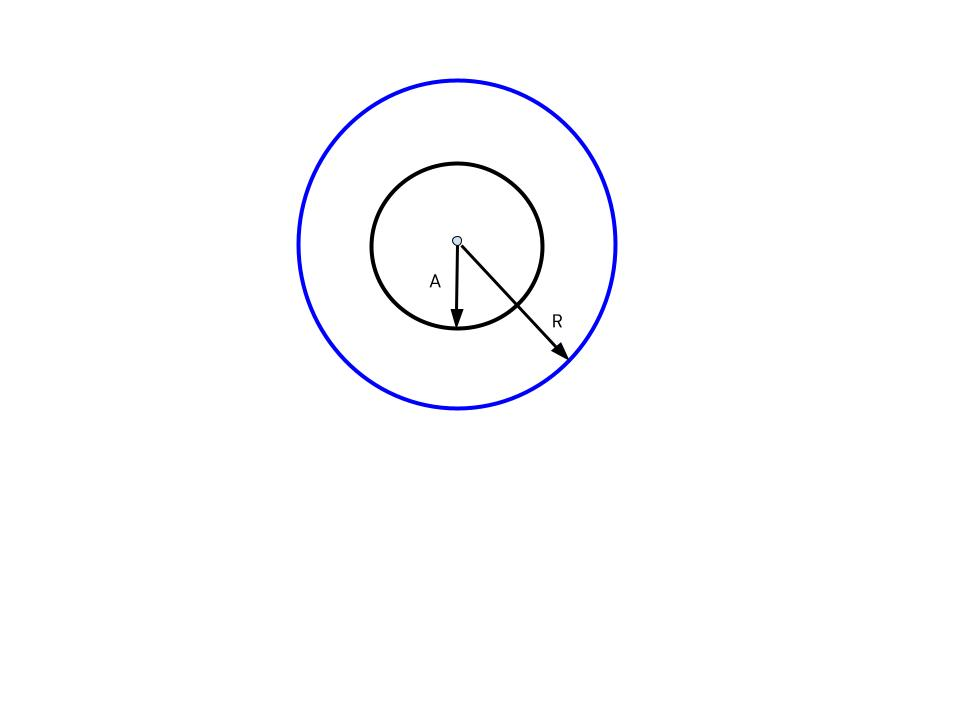
\includegraphics[height = 7cm]{2024-04-18_Diagrama2_ActividadCargas.jpeg}
    \caption{Diagrama de situación en donde $R \geq A$}
    \label{fig:fig2}
\end{figure}
En el diagrama \ref{fig:fig2}, observamos la situación en donde el radio de la carga se ve sobrepasado por el radio de la esfera de la superficie Gaussiana. Análogamente a los procesos anteriores, conviene aplicar las ecuaciones 
\ref{eq:eq1} y \ref{eq:eq2} de la Ley de Gauss. En primer lugar, debido a que la superficie Gaussiana no cambia, la fórmula de $Q_{enc}$ utilizando la integral de superficie sigue siendo la misma, por lo tanto se trae la ecuación \ref{eq:eq6}. Lo que 
quedaría sería resolver la ecuación de $Q_{enc}$ con la integral de volumen, para igualmente igualar éste resultado y el obtenido por medio de la integral de superficie, y despejando,  
obtener una ecuación para la magnitud del campo eléctrico. A continuación se resuelve la integral de volumen: 
\begin{align}
Q_{enc} &= \int \rho_v dv\\ 
Q_{enc} &= \rho v \int (r^2 \sin(\theta) dr d\theta d\phi)\\
Q_{enc} &= \rho_v \int_{0}^{2\pi} d\phi \int_{0}^{\pi}sin(\theta)d\theta \int_{0}^{a} r^2 dr \\
Q_{enc} &= \rho_v [(2\pi - 0)(-1(-(-1)))(\frac{a^3}{3})]\\
Q_{enc} &= \frac{4}{3}\pi a^3 \rho_v \label{eq:eq9}
\end{align}
En el proceso anterior, debido a que la integral de volumen es una integral triple, se separa el diferencial de volumen $dv$ en cada integral correspondiente. En éste caso, $\phi$ va de $0$ a 
$2\pi$, $\theta$ va de 0 a $\pi$, y el radio, a diferencia de la situación anterior, se mueve desde $0$ hasta $a$, $a$ siendo el radio de la superficie Gaussiana. Además, se extrae 
$\rho_v$ debido a que es constante, y por lo tanto se puede extraer de la integral triple. Por lo tanto, la ecuación que nos da la carga encerrada en éste caso es la ecuación 
\ref{eq:eq9}. \\

Gracias a éste resultado, podemos igualar los resultados obtenidos de la integral de volumen (Ecuación \ref{eq:eq9}) y la integral de superficie 
que se mantuvo igual en ambas situaciones (Ecuación \ref{eq:eq6}), para obtener una fórmula que nos permita calcular el campo eléctrico: 
\begin{align}
\frac{4}{3}\pi a^3 \rho_v &= 4\pi r^2 \epsilon_0 E \\
E = \frac{a^3\rho_v}{3\epsilon_0r^2} \label{eq:eq10}
\end{align}
Por lo tanto, la ecuación que nos permite calcular el campo eléctrico es la ecuación \ref{eq:eq10}.\\ Para agregar dirección a ésta fórmula, se agrega el vector unitario $\hat{a}_r$: 
\begin{align}
\vec{E} = \frac{a^3\rho_v}{3\epsilon_0r^2} \cdot \hat{a}_r
\end{align}

A diferencia de la fórmula obtenida para cuando el radio de la superficie 
Gaussiana es menor al radio de la carga (Ecuación \ref{eq:eq7}), aquí la mangitud o intensidad del campo eléctrico disminuye de manera proporcional al $r^2$ o radio de la superficie Gaussiana al cuadrado. Éste 
resultado es interesante ya que nos indica que mientras la superficie Gaussiana crece hasta abarcar la totalidad de la carga, el campo eléctrico aumenta de manera lineal, y una vez que sobrepasa o cubre totalmente 
la carga, disminuye proporcional al radio al cuadrado. \\

\subsection*{Conclusión}
En éste reporte, a partir de la Ley de Gauss se derivaron fórmulas para el campo eléctrico en dos situaciones: La primera cuando el radio de la superficie Gaussiana es menor al radio de la carga, es decir, la superficie 
encierra una parcialidad de la carga, y la segunda cuando el radio de la superficie Gaussiana es mayor al de la carga, es decir, la superficie encierra toda la carga. Se encontraron conclusiones muy interesantes, principalmente que la intensidad 
del campo eléctrico aumenta de manera lineal desde 0 hasta llegar a encerrar la totalidad de la carga, y a partir de ahí el campo eléctrico decrece en intensidad a una tasa 
proporcional al radio al cuadrado de la superficie gaussiana. \\

Por otro lado, cabe destacar el uso de las coordenadas esféricas, que además de facilitar los cálculos, resultan idóneas debido a que la carga de prueba crea el campo eléctrico de manera radial, y por lo tanto, 
para el uso de la Ley de Gauss, una esfera como superficie resulta ideal ya que permite que el campo eléctrico sea perpendicular a la superficie en cualquier punto de ésta. Por lo tanto, es de suma importancia seleccionar 
el sistema de coordenadas correctas dependiendo de la situación, ya sea cartesianas, cilíndricas, o esféricas. \\

Como futuros trabajos basados en éste reporte, sería interesante analizar la situación con una carga negativa, es decir, cuando el flujo eléctrico en la superficie es hacia adentro, y observar el comportamiento del campo 
eléctrico en éstos casos. Otra posible rama de profundización sería analizar la interacción no solo de una carga, sino de 
varias cargas distribuidas en el espacio, lo que puede agregar complejidad pero proporcionar comprensión más profunda. 
\end{document}